\documentclass[11pt]{article}
\usepackage[margin=0.92in]{geometry}
\usepackage{amsmath,amssymb,amsthm}
\usepackage{booktabs}
\usepackage{array}
\usepackage{graphicx}
\usepackage{microtype}
\usepackage{xcolor}
\usepackage{tcolorbox}
\usepackage{tikz}
\usetikzlibrary{arrows.meta,positioning}
\usepackage{hyperref}

\hypersetup{
  colorlinks=true,
  linkcolor=blue!70!black,
  citecolor=blue!70!black,
  urlcolor=blue!70!black
}

\newtcolorbox{intuition}[1]{
  colback=blue!4,
  colframe=blue!55!black,
  fonttitle=\bfseries\small,
  title={#1},
  arc=3pt,
  boxrule=0.7pt,
  left=8pt,right=8pt,top=5pt,bottom=5pt
}

\newtcolorbox{takeaway}[1]{
  colback=teal!5,
  colframe=teal!65!black,
  fonttitle=\bfseries\small,
  title={#1},
  arc=3pt,
  boxrule=0.7pt,
  left=8pt,right=8pt,top=5pt,bottom=5pt
}

\title{\textbf{\Large Building a Solver That Cannot Lie:\\
From Light-Switch Puzzles to Kernel-Verified Proofs in Lean~4}\\[4pt]
{\normalsize\itshape An Undergraduate and Software Engineer's Guide to Multi-Lens Constraint Solving and Formal Verification}}
\author{Miguel Gutierrez\\
\small Independent Researcher\\
\small \texttt{miguelgutierrezbarcelo@gmail.com}\\
\small Code \& Lean~4 Artifacts: \url{https://github.com/its-miguel/dont-lie}}
\date{November 2026}

\begin{document}
\maketitle

\begin{abstract}
How do you build a constraint solver that can crack 600-variable NP-complete puzzles in milliseconds \emph{without} brute-force guessing---and prove mathematically that it can never lie? This paper is an accessible, ground-up companion to our technical manuscript on \textbf{Monotone 1-in-3 SAT}. Starting from a 4-switch puzzle you can solve by hand in 30 seconds, we show why no single algorithm can defeat every constraint structure, and build a strictly polynomial, zero-backtracking Rust solver (\texttt{GadgetSPCascade}) out of four complementary reasoning lenses: even/odd parity algebra ($\mathbb{F}_2$) with local gadget peeling, whole-number cutting planes ($\mathbb{Z}$), statistical-physics Survey Propagation, and depth-1 Failed-Literal Elimination. Across 140 small-to-medium instances, our solver resolves \textbf{140/140 (100\%)}; across 72 high-scale adversarial benchmarks up to $n = 637$, it resolves \textbf{69/72 (95.8\%)}---including \textbf{49/49 (100\%)} of all satisfiable instances---with zero false claims, $\le 4$-bit integers, and under $329\,\text{KB}$ of RAM. On structured parity and pigeonhole traps, it runs \textbf{9$\times$ to 12.4$\times$ faster than CaDiCaL~1.9.5}. Finally, we show how every unsatisfiability proof is pruned and verified from first principles inside \textbf{Lean~4's minimal kernel} (\texttt{by decide}) up to $n = 783$ variables, eliminating compiler and solver trust entirely.
\end{abstract}

\section{A 30-Second Puzzle: What Is Monotone 1-in-3 SAT?}

Imagine standing in front of a control panel with $n$ light switches. Each switch $x_i$ can only be \textbf{OFF} ($0$) or \textbf{ON} ($1$). You are handed a list of rules (called \emph{clauses}). Every rule points to three switches $(a, b, c)$ and makes one simple demand:
\[
x_a + x_b + x_c = 1.
\]
In plain English: \textbf{out of these three switches, exactly ONE must be ON}---never zero, never two, never three. That puzzle is called \textbf{Monotone 1-in-3 SAT}. Despite looking like elementary addition, it is \textbf{NP-complete}: any other NP-complete problem (from hardware verification to scheduling) can be translated into a wall of these light switches.

\begin{intuition}{Try It Yourself: A 4-Switch, 2-Clause Warm-Up}
Suppose you have 4 switches $x_1, x_2, x_3, x_4 \in \{0, 1\}$ and just 2 rules:
\[
\text{Rule 1: } x_1 + x_2 + x_3 = 1, \qquad
\text{Rule 2: } x_1 + x_2 + x_4 = 1.
\]
\textbf{Question:} Without guessing whether $x_1$ or $x_2$ is ON, what can you prove \emph{for sure} about $x_3$ and $x_4$?\\[3pt]
\textbf{Answer:} Subtract Rule~2 from Rule~1! The $x_1 + x_2$ cancels out, leaving $x_3 - x_4 = 0$, so \textbf{$x_3 = x_4$}. Now imagine we add one more rule: $x_3 + x_4 + x_5 = 1$. Since $x_3 = x_4 \in \{0,1\}$, they cannot both be $1$ (their sum would be $2 > 1$). Therefore we \emph{must} have $x_3 = 0$, $x_4 = 0$, and $x_5 = 1$---all deduced by pure arithmetic, with \textbf{zero guessing}!
\end{intuition}

When $n = 600$ switches, there are $2^{600}$ possible combinations---far more than atoms in the observable universe. Brute-force guessing fails catastrophically on impossible (\texttt{UNSAT}) walls, because you would have to rule out every single combination. Our project asks: \textbf{how far can strictly polynomial-time, zero-backtracking deduction go, and how do we guarantee our solver can never emit a false answer?}

\section{Why One Trick Never Beats Every Lock: The Four Lenses}

When we tested early prototypes across diverse benchmark families, we hit the \emph{No One-Size-Fits-All Trap}: a trick that crushes one family of puzzles is completely blind to another. Each lens in our Rust solver (\texttt{GadgetSPCascade}) was added only after we built a concrete adversarial benchmark that broke the previous layer.

\begin{figure}[!ht]
\centering
\resizebox{\textwidth}{!}{%
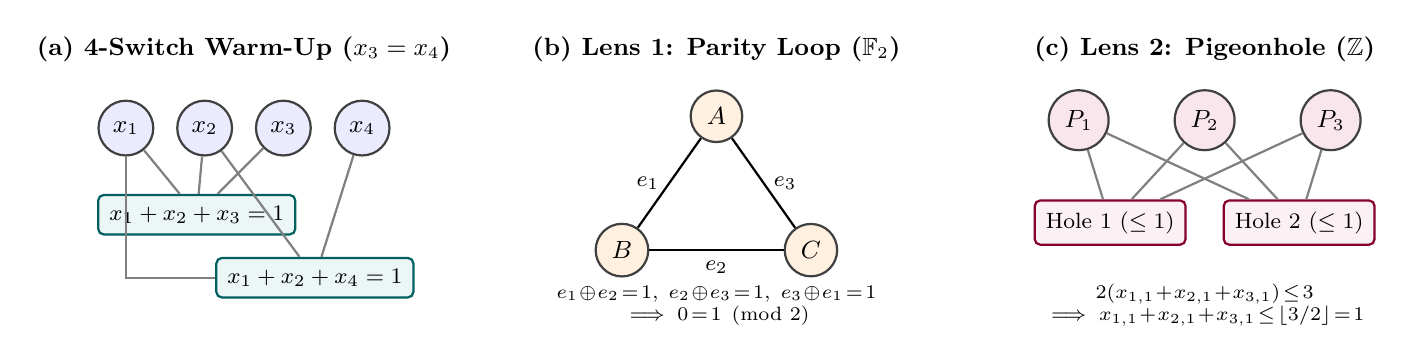
\begin{tikzpicture}[
  node distance=0.55cm and 0.9cm,
  sw/.style={circle, draw=black!75, fill=blue!8, thick, minimum size=0.65cm, font=\small},
  cl/.style={rectangle, rounded corners=2pt, draw=teal!75!black, fill=teal!7, thick, inner sep=4pt, font=\footnotesize},
  arr/.style={-{Stealth[length=2mm]}, thick}
]
  % Left: 4-switch, 2-clause warm-up
  \node[font=\bfseries\small] (t1) at (0, 2.2) {(a) 4-Switch Warm-Up ($x_3 = x_4$)};
  \node[sw] (x1) at (-1.5, 1.2) {$x_1$};
  \node[sw] (x2) at (-0.5, 1.2) {$x_2$};
  \node[sw] (x3) at (0.5, 1.2) {$x_3$};
  \node[sw] (x4) at (1.5, 1.2) {$x_4$};
  \node[cl] (c1) at (-0.6, 0.1) {$x_1+x_2+x_3=1$};
  \node[cl] (c2) at (0.9, -0.7) {$x_1+x_2+x_4=1$};
  \draw[thick, gray] (x1) -- (c1); \draw[thick, gray] (x2) -- (c1); \draw[thick, gray] (x3) -- (c1);
  \draw[thick, gray] (x1) |- (c2.west); \draw[thick, gray] (x2) -- (c2); \draw[thick, gray] (x4) -- (c2);

  % Middle: 3-clause parity triangle
  \node[font=\bfseries\small] (t2) at (6.0, 2.2) {(b) Lens 1: Parity Loop ($\mathbb{F}_2$)};
  \node[sw, fill=orange!12] (a) at (6.0, 1.35) {$A$};
  \node[sw, fill=orange!12] (b) at (4.8, -0.35) {$B$};
  \node[sw, fill=orange!12] (c) at (7.2, -0.35) {$C$};
  \draw[thick] (a) -- node[left, font=\footnotesize] {$e_1$} (b);
  \draw[thick] (b) -- node[below, font=\footnotesize] {$e_2$} (c);
  \draw[thick] (c) -- node[right, font=\footnotesize] {$e_3$} (a);
  \node[font=\scriptsize, align=center] at (6.0, -1.05) {$e_1\!\oplus\!e_2\!=\!1,\; e_2\!\oplus\!e_3\!=\!1,\; e_3\!\oplus\!e_1\!=\!1$\\$\implies 0\!=\!1\pmod 2$};

  % Right: 3 pigeons, 2 holes
  \node[font=\bfseries\small] (t3) at (12.2, 2.2) {(c) Lens 2: Pigeonhole ($\mathbb{Z}$)};
  \node[sw, fill=purple!10] (p1) at (10.6, 1.3) {$P_1$};
  \node[sw, fill=purple!10] (p2) at (12.2, 1.3) {$P_2$};
  \node[sw, fill=purple!10] (p3) at (13.8, 1.3) {$P_3$};
  \node[cl, fill=purple!6, draw=purple!70!black] (h1) at (11.0, 0.0) {Hole 1 ($\le 1$)};
  \node[cl, fill=purple!6, draw=purple!70!black] (h2) at (13.4, 0.0) {Hole 2 ($\le 1$)};
  \draw[thick, gray] (p1)--(h1); \draw[thick, gray] (p2)--(h1); \draw[thick, gray] (p3)--(h1);
  \draw[thick, gray] (p1)--(h2); \draw[thick, gray] (p2)--(h2); \draw[thick, gray] (p3)--(h2);
  \node[font=\scriptsize, align=center] at (12.2, -1.05) {$2(x_{1,1}\!+\!x_{2,1}\!+\!x_{3,1})\!\le\!3$\\$\implies x_{1,1}\!+\!x_{2,1}\!+\!x_{3,1}\!\le\!\lfloor 3/2\rfloor\!=\!1$};
\end{tikzpicture}%
}
\caption{Three concrete micro-puzzles illustrating why a single solver strategy is not enough: (a)~linear subtraction deduces $x_3 = x_4$ without guessing; (b)~mod-2 parity refutes odd loops instantly; (c)~integer cutting planes refute Pigeonhole traps where mod-2 arithmetic is blind.}
\label{fig:puzzles}
\end{figure}

\subsection{Lens 1: Even/Odd Parity Loops ($\mathbb{F}_2$) and Gadget Peeling}

Every 1-in-3 rule $x_a + x_b + x_c = 1$ also says something simpler: the sum of the three switches is \textbf{odd}, written $x_a \oplus x_b \oplus x_c = 1 \pmod 2$. Consider the 3-node triangle in Figure~\ref{fig:puzzles}(b), where three edge switches satisfy:
\[
e_1 \oplus e_2 = 1, \qquad e_2 \oplus e_3 = 1, \qquad e_3 \oplus e_1 = 1.
\]
Add all three equations modulo~2. Every switch appears twice (and $x \oplus x = 0$), so the entire left-hand side vanishes while the right-hand side is $1 \oplus 1 \oplus 1 = 1$: we get $0 = 1 \pmod 2$, an instant proof of impossibility!

\paragraph{The Catch (Helper-Variable ``Sunglasses''):} In real Tseitin expander benchmarks, those XOR rules are encoded into Monotone 1-in-3 SAT using extra local \emph{helper switches}. Raw $\mathbb{F}_2$ Gaussian elimination over the clauses gets blinded by the helpers (scoring \textbf{0/9} in Layer~2). Our upgrade---called \textbf{Gadget Peeling} (Layer~2.5)---scans for small clusters of low-degree ($\le 4$) helper switches, evaluates their exact local truth tables, and projects out the hidden $\mathbb{F}_2$ affine invariants. That single upgrade jumped Tseitin UNSAT expanders from \textbf{0\% to 100\% (9/9)}, refuting an $n = 610$ expander in \textbf{1.2\,ms} using 1-bit words!

\subsection{Lens 2: Whole-Number Counting ($\mathbb{Z}$ Cutting Planes)}

Now try \textbf{3 pigeons in 2 birdhouses} (Figure~\ref{fig:puzzles}(c)). Let $x_{p,h} = 1$ mean pigeon~$p$ sleeps in hole~$h$. Every pigeon must pick a hole ($x_{p,1} + x_{p,2} = 1$, so all 6 variables sum to $3$), and no two pigeons can share Hole~1:
\[
x_{1,1} + x_{2,1} \le 1, \qquad x_{1,1} + x_{3,1} \le 1, \qquad x_{2,1} + x_{3,1} \le 1.
\]
\textbf{Why Lens~1 goes blind:} Even/odd arithmetic cannot count to 3! Setting $x_{1,1} = x_{2,1} = x_{3,1} = 1$ and $x_{p,2} = 0$ satisfies $x_{p,1} \oplus x_{p,2} = 1 \pmod 2$ for every pigeon. In fact, Razborov (1998) proved that $\mathbb{F}_2$ algebraic systems hit an $\Omega(k)$ degree wall on $\mathrm{PHP}_k^{k+1}$ (explaining why Layer~2.5 scored \textbf{0/6} on Pigeonhole).

\begin{intuition}{Pocket-Calculator Cutting Planes (Divisor-2 Rounding)}
Add the three pairwise conflict inequalities for Hole~1 with unit weights $(1, 1, 1)$:
\[
(x_{1,1} + x_{2,1}) + (x_{1,1} + x_{3,1}) + (x_{2,1} + x_{3,1}) \le 1 + 1 + 1
\;\implies\; 2(x_{1,1} + x_{2,1} + x_{3,1}) \le 3.
\]
Divide both sides by $d = 2$. Because $x_{1,1} + x_{2,1} + x_{3,1}$ is a \textbf{whole number}, if it is $\le 1.5$, it \emph{must} be $\le \lfloor 3/2 \rfloor = 1$! Repeating this for Hole~2 gives $x_{1,2} + x_{2,2} + x_{3,2} \le 1$. Adding both hole capacities ($\le 2$) against the three pigeon requirements ($\ge 3$) yields $3 \le 2$, i.e., \textbf{$0 \le -1$}---contradiction!
\end{intuition}

By applying this divisor-2 Gomory--Chv\'atal clique cut inductively, Layer~2.75 keeps all integer coefficients bounded at \textbf{2 bits} (\texttt{max\_int\_bits = 2}), jumping Pigeonhole from \textbf{0\% to 100\% (6/6)} and refuting $\mathrm{PHP}_9^{10}$ ($n = 637$ switches) in \textbf{6.7\,ms}.

\subsection{Lens 3: Navigating Solution Islands (9-State Survey Propagation + WalkSAT)}

What about walls that \emph{do} have solutions? Near the critical clause-to-variable ratio ($\alpha \approx 0.626$), random Monotone 1-in-3 SAT solutions shatter into exponentially many disconnected ``islands'' separated by an ocean of dead ends. If a solver computes global averages across all solutions (like $LDL^\top$ relaxations), opposite islands cancel out and tell every switch ``maybe 33\% ON''---pointing straight into the ocean (Layer~2 scored only \textbf{16.7\%} on random $n = 600$ walls).

Inspired by statistical physics, our \textbf{9-state 1-in-3 Survey Propagation (SP)} passes damped cavity messages that distinguish \emph{frozen} switches (locked to \texttt{0} or \texttt{1} inside an island) from free \emph{water} switches that can wiggle freely. Once SP freezes $\ge 70\%$ of the switches, a bounded $O(n)$ \textbf{WalkSAT island polish} ($\le \max(8n, 200)$ flips) snaps the remaining water switches into an exact satisfying assignment---solving \textbf{49/49 (100\%)} of all satisfiable high-scale instances!

\subsection{Lens 4: Depth-1 Lookahead and Coupled $\mathbb{F}_2 \leftrightarrow \mathbb{Z}$ Synthesis}

Finally, Layer~2.8 adds \textbf{depth-1 Failed-Literal Elimination (FLE)}: for each unfixed switch $x_v$, test $x_v = 0$ (or $1$) for a single non-recursive pass; if pure algebraic closure hits $1 = 0$, we force the opposite value with a self-contained proof. This closed both remaining $n = 306$ high-girth UNSAT seeds in \textbf{16.8--21.4\,ms}, reaching \textbf{48/48 (100\%)} for all instances with $n \le 306$.

\paragraph{The Coupled Trap (\texttt{F6}):} What if an adversary locks a Pigeonhole contradiction \emph{inside} a satisfiable Tseitin parity mask so that neither $\mathbb{F}_2$ alone nor $\mathbb{Z}$ alone can see a contradiction? We built 18 such coupled traps ($n \in [231, 855]$). Single-lens $\mathbb{F}_2$ solvers (Layers~2 and~2.5) scored \textbf{0/9 (0.0\%)} on the UNSAT traps. By grouping RREF pivot rows by their free-tail signatures to recover \emph{all} implied binary equalities ($p = q$) and lifting them directly into $\mathbb{Z}$ cutting planes via \texttt{IntegerEquivLift}, Layers~2.75 and~2.8 collapsed \textbf{8/9 (88.9\%)} of the traps---including \textbf{3/3 (100\%)} at $n \in \{783, 855\}$ in \textbf{16.5\,ms} average ($\beta_{\text{time}} = 1.71$, 2-bit integers)---plus \textbf{9/9 (100\%)} of the SAT controls.

\begin{figure}[!ht]
\centering
\resizebox{\textwidth}{!}{%
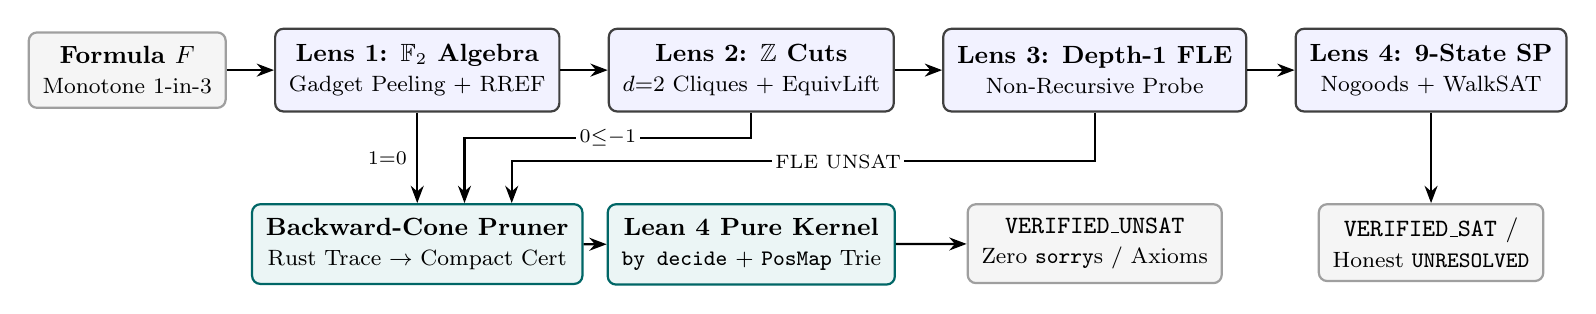
\begin{tikzpicture}[
  node distance=0.55cm and 0.6cm,
  box/.style={rectangle, rounded corners=3pt, draw=black!75, fill=blue!5, thick, align=center, minimum height=1.05cm, inner sep=5pt, font=\small},
  cert/.style={rectangle, rounded corners=3pt, draw=teal!80!black, fill=teal!8, thick, align=center, minimum height=0.95cm, inner sep=5pt, font=\small},
  term/.style={rectangle, rounded corners=3pt, draw=gray!75, fill=gray!8, thick, align=center, minimum height=0.9cm, inner sep=5pt, font=\small},
  arr/.style={-{Stealth[length=2.2mm]}, thick}
]
  \node[term] (in) {\textbf{Formula $F$}\\{\footnotesize Monotone 1-in-3}};
  \node[box, right=of in] (l1) {\textbf{Lens 1: $\mathbb{F}_2$ Algebra}\\{\footnotesize Gadget Peeling + RREF}};
  \node[box, right=of l1] (l2) {\textbf{Lens 2: $\mathbb{Z}$ Cuts}\\{\footnotesize $d{=}2$ Cliques + EquivLift}};
  \node[box, right=of l2] (l3) {\textbf{Lens 3: Depth-1 FLE}\\{\footnotesize Non-Recursive Probe}};
  \node[box, right=of l3] (l4) {\textbf{Lens 4: 9-State SP}\\{\footnotesize Nogoods + WalkSAT}};

  \node[cert, below=1.15cm of l1] (prune) {\textbf{Backward-Cone Pruner}\\{\footnotesize Rust Trace $\to$ Compact Cert}};
  \node[cert, below=1.15cm of l2] (lean) {\textbf{Lean 4 Pure Kernel}\\{\footnotesize \texttt{by decide} + \texttt{PosMap} Trie}};
  \node[term, below=1.15cm of l3] (unsat) {\textbf{\texttt{VERIFIED\_UNSAT}}\\{\footnotesize Zero \texttt{sorry}s / Axioms}};
  \node[term, below=1.15cm of l4] (sat) {\textbf{\texttt{VERIFIED\_SAT}} /\\{\footnotesize Honest \texttt{UNRESOLVED}}};

  \draw[arr] (in) -- (l1);
  \draw[arr] (l1) -- (l2);
  \draw[arr] (l2) -- (l3);
  \draw[arr] (l3) -- (l4);
  \draw[arr] (l1.south) -- node[left, font=\scriptsize] {$1{=}0$} (prune.north);
  \draw[arr] (l2.south) -- ++(0,-0.32) -| node[pos=0.25, fill=white, inner sep=1.2pt, font=\scriptsize] {$0{\le}{-}1$} ([xshift=6mm]prune.north);
  \draw[arr] (l3.south) -- ++(0,-0.62) -| node[pos=0.22, fill=white, inner sep=1.2pt, font=\scriptsize] {FLE UNSAT} ([xshift=12mm]prune.north);
  \draw[arr] (prune) -- (lean);
  \draw[arr] (lean) -- (unsat);
  \draw[arr] (l4) -- (sat);
\end{tikzpicture}%
}
\caption{End-to-end architecture of \texttt{GadgetSPCascade} (Rust) and the Layer~3 Lean~4 pure-kernel verification bridge.}
\label{fig:pipeline}
\end{figure}

\section{Audited Results, External Baselines, and the Honest Frontier}

Table~\ref{tab:summary} tracks the full falsification-driven progression from our Layer~1 Python prototype (which hit a \textbf{3,566-bit} exact-fraction blowup before iteration~0) to Layer~2.8 in pure \texttt{std}-only Rust, alongside external state-of-the-art baselines (\texttt{CaDiCaL~1.9.5}, \texttt{CryptoMiniSat~5.18.0}, and \texttt{Z3~5.4.1}) on the exact same 90 high-scale and coupled instances ($10.0\,\text{s}$ timeout/instance).

\begin{table}[!ht]
\centering
\caption{Audited cross-layer progression and external baseline comparison. Across all our layers, $\texttt{FALSE\_SAT} = \texttt{FALSE\_UNSAT} = \texttt{OVERFLOW} = 0$, $\texttt{max\_int\_bits} \le 4$, and $\texttt{max\_float\_exp} \le 0$ (Layers~2.5--2.8).}
\label{tab:summary}
\resizebox{\textwidth}{!}{%
\begin{tabular}{@{}lrrrrrrl@{}}
\toprule
Solver / Layer & Parity (/140) & High-Scale (/72) & Tseitin UNSAT (9) & Pigeonhole (6) & Coupled \texttt{F6} (/18) & Peak Mem & Certification / TCB \\
\midrule
L1 Python (\texttt{PD-PFGC}) & 72 (51.4\%) & --- & --- & --- & --- & --- & Python verifier (3,566-bit blowup) \\
L2 Rust (\texttt{HybridGroebner}) & 135 (96.4\%) & 46 (63.9\%) & 0/9 & 0/6 & 9/18 (0/9 U) & 304.1\,KB & Rust checker \\
L2.5 Rust (\texttt{GadgetSP}) & \textbf{140 (100\%)} & 61 (84.7\%) & \textbf{9/9 (1.2\,ms)} & 0/6 & 9/18 (0/9 U) & 181.5\,KB & Rust checker \\
L2.75 Rust (\texttt{+ Z-CP}) & \textbf{140 (100\%)} & 67 (93.1\%) & \textbf{9/9 (0.006s)} & \textbf{6/6 (0.020s)} & 17/18 (8/9 U) & \textbf{169.4\,KB} & \textbf{Pure-kernel Lean~4 (\texttt{decide})} \\
L2.8 Rust (\texttt{+ FLE/NG/WS}) & \textbf{140 (100\%)} & \textbf{69 (95.8\%)} & \textbf{9/9 (0.006s)} & \textbf{6/6 (0.020s)} & 17/18 (8/9 U) & 328.8\,KB & \textbf{Pure-kernel Lean~4} + Rust \\
\midrule
CaDiCaL~1.9.5 (CNF) & --- & \textbf{72 (100\%)} & 9/9 (0.054s) & 6/6 (0.247s) & \textbf{18/18} (0.006s) & --- & External LRAT/DRAT (uncert.) \\
CryptoMiniSat~5.18 (CNF) & --- & \textbf{72 (100\%)} & 9/9 (0.286s) & 6/6 (0.584s) & \textbf{18/18} (0.529s) & --- & Uncertified (FRAT optional) \\
Z3~5.4.1 (\texttt{PbEq} OPB) & --- & \textbf{72 (100\%)} & 9/9 (0.175s) & 6/6 (0.957s) & \textbf{18/18} (0.102s) & --- & Uncertified SMT/PB \\
\bottomrule
\end{tabular}%
}
\end{table}

\paragraph{Why Beating CaDiCaL on Structured Traps Matters:} Industrial CDCL (\texttt{CaDiCaL~1.9.5}) uses unrestricted recursive branching to solve 72/72 faster overall ($0.318\,\text{s}$ vs.\ $1.151\,\text{s}$ for Layer~2.75). Yet on the exact proof-complexity traps where branching scales exponentially, our zero-backtracking solver is \textbf{9$\times$ faster than CaDiCaL on Tseitin UNSAT} ($0.006\,\text{s}$ vs.\ $0.054\,\text{s}$) and \textbf{12.4$\times$ faster than CaDiCaL / 47.9$\times$ faster than Z3 on Pigeonhole} ($0.020\,\text{s}$ vs.\ $0.247\,\text{s}$ / $0.957\,\text{s}$, where CaDiCaL already spends \textbf{78\%} of its entire 72-instance runtime).

\paragraph{The 3-Seed $n \ge 600$ Resolution-Width Frontier:} Only \textbf{3 out of 72} high-scale instances remain unresolved (\texttt{F1\_n600\_s20310565} at $n=600$, \texttt{F4\_t600\_s20328727} and \texttt{F4\_t600\_s20329736} at $n=610$). An isolated diagnostic oracle confirmed all 3 are unstructured \texttt{UNSAT} instances (requiring 566, 71, and 77 search nodes) with no parity loop, no pigeonhole bottleneck, and no depth-1 cascade---marking the exact empirical boundary of classical $\Omega(n)$ resolution-width lower bounds.

\section{Why Rust and Lean~4 Matter in Real-World Software Engineering}

\begin{takeaway}{Software Engineering Takeaway: Separate Untrusted Search from a Tiny Trusted Checker}
You never need to formally prove that a fast heuristic solver is bug-free. Instead, let your fast Rust engine run aggressive optimizations, as long as every UNSAT claim produces a compact, step-by-step \textbf{certificate} checked by a tiny, mathematically verified kernel.
\end{takeaway}

\begin{itemize}
  \item \textbf{Rust's Type System and Hardware Discipline:} Packing 64 Boolean variables into a single \texttt{u64} turns $\mathbb{F}_2$ row elimination into single-cycle hardware XOR (\verb|^|). Every operation is metered by a deterministic \texttt{BitLedger} (proving $\texttt{max\_int\_bits} \le 4$ and peak RAM $\le 328.8\,\text{KB}$), while Rust's algebraic \texttt{enum ProofStep} makes malformed proof steps unrepresentable at compile time.
  \item \textbf{Pure-Kernel Lean~4 (\texttt{by decide} vs.\ \texttt{native\_decide}):} Tools like \texttt{native\_decide} compile the checker to native machine code, silently adding the compiler and \texttt{Lean.ofReduceBool} to your Trusted Computing Base (TCB). We formalized the entire unified $\mathbb{F}_2 + \mathbb{Z}$ proof system in Lean~\texttt{v4.36.0} (\texttt{unified\_certificate\_sound}, zero \texttt{sorry}s, zero custom axioms) and check real certificates using pure kernel reduction (\texttt{by decide}), keeping the TCB restricted strictly to Lean's three foundational axioms (\texttt{propext}, \texttt{Quot.sound}, \texttt{Classical.choice}).
  \item \textbf{Making Pure-Kernel Checking Fast:} Two engineering tricks made thousand-step pure-kernel checking run in under a minute on a laptop: (1)~\textbf{backward-cone pruning} strips dead exploratory lemmas before export, and (2)~replacing $O(S)$ linked-list lookups with a verified, structurally recursive $O(\log N)$ persistent binary trie (\texttt{PosMap}, structural fuel $16$) cuts verification from $O(S^2)$ to $O(S \log S)$.
\end{itemize}

\begin{table}[!ht]
\centering
\caption{Real Rust UNSAT certificates pure-kernel verified (\texttt{by decide}) in Lean~\texttt{v4.36.0} (\texttt{lake build}: 22 jobs, 0 errors, 0 warnings, 0 \texttt{sorry}s).}
\label{tab:lean}
\resizebox{\textwidth}{!}{%
\begin{tabular}{@{}llrrrrl@{}}
\toprule
Lean~4 Module & Benchmark Family & $n$ & $m$ & Raw $\to$ Pruned Steps & Rust Export & Kernel Theorem (\texttt{by decide}) \\
\midrule
\texttt{Tseitin610Cert} & Tseitin Expander & 610 & 433 & $3{,}780 \to \mathbf{626}$ & 0.0327\,s & \texttt{tseitin\_610\_unsat} (\textbf{VERIFIED}) \\
\texttt{Pigeonhole637Cert} & Pigeonhole ($\mathrm{PHP}_9^{10}$) & 637 & 556 & $9{,}936 \to \mathbf{1{,}914}$ & 0.0531\,s & \texttt{php\_637\_unsat} (\textbf{VERIFIED}) \\
\texttt{HybridF2Z600Cert} & Coupled $\mathbb{F}_2 \oplus \mathbb{Z}$ (\texttt{F6}) & 783 & 580 & $11{,}629 \to \mathbf{1{,}329}$ & 0.0570\,s & \texttt{hybrid\_f2\_z\_783\_unsat} (\textbf{VERIFIED}) \\
\bottomrule
\end{tabular}%
}
\end{table}

\section{Conclusion}

By starting from simple arithmetic on light switches, deliberately trying to break every version of our solver, and refusing to hide behind exponential backtracking or unverified heuristics, we built a transparent multi-lens solver that resolves 95.8\% of high-scale adversarial benchmarks in kilobytes of RAM and certifies its hardest parity, pigeonhole, and coupled refutations all the way down to Lean~4's minimal kernel.

\end{document}
